%!TEX root = CS_ORNs.tex

Animals can identify and discriminate a myriad of odors using a surprisingly limited class of distinct olfactory receptor genes. It was recently noted that a critical feature of our odor environment may resolve this inconsistency: most naturally-occurring odors are composed of only a tiny subset of these many volatile molecular constituents~\cite{vijay_1}. In principle, the high-dimensional odor signal could be accurately decompressed from a limited number of receptor measurements, provided (i) the odor signal is sufficiently sparse in odorant space and (ii) the responses are sufficiently dispersed. The latter requires that odor receptors are not odorant-specific but bind many odorants with distinct affinities, and that a given odorant elicits responses in several such receptors. Odor identity is therefore coded in the unique combination of responses the odor elicits in the sensing repertoire -- a combinatorial coding strategy. 

Transformations of olfactory receptor neuron (ORN) response in the subsequent neural circuitry lends further credence to a combinatorial coding strategy. In \textit{Drosophila}, ORNs in the periphery synapse to neuropil compartments in the antennal lobe called glomeruli (ORNs expressing a given Or synapse to the same glomerulus), where they then divergently and randomly synapse to Kenyon cells in the mushroom body (MB) and lateral horn~\cite{early_olfactory_processing, abbott_axel}. In the MB, the responses are decoded and sent to higher order brain centers where they are translated to behavioral response~\cite{olfactory_map_chiang, mushroom_body_review}. It has been suggested that in a combinatorial coding strategy, this dispersion of ORN response along the olfactory pathway from AL to MB may further facilitate flexible learning and robust odor discrimination~\cite{vijay_1}. Indeed, this response diffusivity has been observed in ORNs in the  \textit{Drosophila melanogaster} sensing periphery~\cite{hallem_carlson}. 

Combinatorial coding relies fundamentally on randomness in the matrix of response, and one potential complication in this coding paradigm is response saturation. Maximum ORN firing rates increase with single odorant concentration rather inhomogenously, potentially jeopardizing response breadth as odor concentrations change. ORNs expressing the receptor Or35a, for example, fire at varying rates spanning 30 to 300 Hz in response to one of eleven distinct odorants at dilutions of $10^{-4}$~\cite{hallem_carlson}. But at dilutions of $10^{-2}$, these maximum rates have all elevated to a narrow range between 200 and 250 Hz
. Similar apparent saturation occurs for ORNs expressing Or85b, Or22a, and OR67a in response to the same panel of odorants. {\color{blue} Discuss natural statistics odors fluctuating.} {\color{blue} Discuss the statistics changings}

On the other hand, it has been shown that ORN local field potentials and firing rates adapt to odor stimuli in time~\cite{martelli, srinivas_elife, cao_WL}. Specifically, it has been shown that in response to single odorant pulses, \textit{Drosophila}  ORN firing rate gain scales inversely with mean odor concentration, according to the Weber-Fechner law observed in vision~\cite{cao_WL, cafaro_WL, srinivas_elife}. This observed scaling law was obeyed by all the odorant-ORN pairs tested, pointing to a mechanistic origin involving the universal co-receptor Orco. Further implicating Orco in gain modulation is the observation that Orco dephosphorylizes following prolonged exposure to odors, leading to receptor desensitization~\cite{Guo_Smith_review, Guo_Smith}. 

Here, we incorporate these findings into a biophysical model that combines odor transduction and receptor activity in the \textit{Drosophila} olfactory periphery with a neural framework for decoding distributed ORN responses. We find that front-end adaptation enacted through the Weber-Fechner Law preserves odor identification across wide variations in odor intensity, and maintains odor discrimination accuracy in conflicting environments. Further, we find that this adaptive mechanism promotes active odor perception in temporally dynamic odor landscapes and among conflicting odor backgrounds. Together, our findings suggest a fundamental role for input gain control in maintaining olfactory sensitivity within naturalistic odor environments. 






\section{Results}



%%%%%%%%%%%%%%%%%%%%%%%%%%%%%%%%%%%%%%%%%%%%%%%%%%%%%%%%%%%%%%%%%
%%%%%%%%%%%%    		MODEL DESCRIPTION    		%%%%%%%%%%%%%
%%%%%%%%%%%%%%%%%%%%%%%%%%%%%%%%%%%%%%%%%%%%%%%%%%%%%%%%%%%%%%%%%



\subsection{A model of odor encoding that preserves the diversity of ORN response and adaptive scaling}


The framework of odor discrimination consists of two stages: odor transduction and subsequent ORN activity (encoding), and a paradigm for then inferring odor identity from this repertoire of ORN response (decoding). The encoding model is a generalization of one recently used to describe front-end adaptation in individual \textit{Drosophila} ORNs~\cite{srinivas_elife}. There, the observed generality of Weber's Law (it was demonstrated in xx odorant/receptor pairs) implicates structural modification of the universal co-receptor Orco, rather than odorant-specific Ors alone. Here, we generalize this model to a repertoire of $a$ ORNs, each housing a collection of Or/Orco complexes. These complexes bind and unbind odorant molecules stochastically, and are assumed to reside in either an active (open ion channel) or inactive state. In equilibrium, a given odorant-receptor pair ($i$-$a$) depends on two disassociation constants, $K^*_{ia}$ and $K_{ia}$, for odorant binding in the active and inactive conformations, respectively. Together, these comprise a coupled stochastic system that translates the binding of odors of varying identities and concentrations into a repertoire of ORN response (Fig.~\ref{fig:tuning_curves_a}). In steady state, the active fraction $\bar A_a$ of Or/Orco complexes in ORN $a$ is:
\begin{align}
\bar{A}_a = \left(1 + e^{\epsilon_a}\frac{1 + \sum_i^N s_i/K_{ia}}{1 + \sum_i^N s_i/K^*_{ia}}\right)^{-1},
\label{eq:steady_state_act}
\end{align}
where $s_i$ is the concentration of the odorant $i$, $i~=~1,...,N$. Odors bind to active Or/Orco complexes much faster than to inactive complexes, whereby $K^*_{ia}~\ll~K_{ia}$. In the case of a mono-molecular odor ($N~=~1$), Weber's Law can be satisfied exactly if the complex activation energy scales logarithmically with the odor concentration, $\epsilon_a \sim \ln s_i$. For an odor with several molecular constituents at distinct concentrations, we instead scale the energy with the mean odorant concentration, $\epsilon_a \sim \ln \langle s_i \rangle$, the average being taken over all non-zero concentrations $s_i$ . Finally, we assume that the free energies modulate only within a finite range, $\epsilon_{\text {L}} < \epsilon_a < \epsilon_{\text {H}}$.




%%%%%%%%%%%%%%%%%%%%%%%%%%%%%%%%%%%%%%%%%%%%%%%%%%%%%%%%%%%%%%%%%
%%%%%%%%%%%%		TUNING CURVES FIGURE			%%%%%%%%%%%%%
%%%%%%%%%%%%%%%%%%%%%%%%%%%%%%%%%%%%%%%%%%%%%%%%%%%%%%%%%%%%%%%%%




\begin{figure*}[!tb]
	\centering
	\begin{subfigure}[t]{0.85\linewidth}
		\phantomsubcaption
		\label{fig:tuning_curves_a}
	\end{subfigure}
	\begin{subfigure}[t]{0\linewidth}
		\phantomsubcaption
		\label{fig:tuning_curves_b}
	\end{subfigure}
	\begin{subfigure}[t]{0\linewidth}
		\phantomsubcaption
		\label{fig:tuning_curves_c}
	\end{subfigure}
	\begin{subfigure}[t]{0\linewidth}
		\phantomsubcaption
		\label{fig:tuning_curves_d}
	\end{subfigure}
	\begin{subfigure}[t]{0\linewidth}
		\phantomsubcaption
		\label{fig:tuning_curves_e}
	\end{subfigure}
	\begin{subfigure}[t]{0\linewidth}
		\phantomsubcaption
		\label{fig:tuning_curves_f}
	\end{subfigure}
	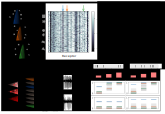
\includegraphics[width=\textwidth]{figures/Figures_tuning_curve}
	\caption{\footnotesize{
		\textbf{A}~Odor binding model. Odorants bind to Or/Orco complexes, which may be quiescent (light gray) or active (dark gray). The likelihood that a complex is in an active state depends on its binding affinity to constituent odor molecules (through $K^*_{i, a}$) and the energetic cost of receptor activation. 
		\textbf{B}~Or classes exhibit distinct binding distributions. 
		\textbf{C}~Example instantiation of the active binding disassociation matrix $K^*_{i, a}$ (see Methods). 
		\textbf{D}~Sample Or/Orco activity of 9 of the 40 ORNs represented by the matrix in (C). The tuning curves, individually ordered by odorant for visualization, exhibit broad, specialized, and weak responses. 
		\textbf{E}~Schematic of Weber Law feedback at signal transduction. When Weber Law is enforced, activity distributions of active complexes (shaded darkly) remain invariant with increasing signal concentrations. 
		\textbf{F}~Steady state Or/Orco activity for the three sample ORNs in (B), (C), and (D), in an unadaptive system (top row) and adaptive system (bottom row) in response to 100 different sparse odors; each matrix row corresponds to a distinct odor identity. The variance of Or/Orco activity across odor identity can rapidly diminish in the absence of front-end adaptation (final column).
		}}
	\label{fig:tuning_curves}
\end{figure*}

Ignoring for the moment the slower effects of adaptation (i.e., assuming $\epsilon_a$ is fixed), this model represents the instantaneous change in the activity as a function of ligand concentration, i.e. similar to the maximum firing rate measured in~\cite{hallem_carlson}. We first show that the steady state response reproduce the diversity of observed ORN tuning curves. Olfactory receptors in \textit{Drosophila} can range from narrowly tuned, responding to a single odorant, to quite broad, responding to various distinct odorants spanning multiple functional groups. We incorporate this diversity of response into our framework by treating $K^*_{ia}$ and $K_{ia}$ as random variables with pre-defined statistics. Figures~\ref{fig:tuning_curves_b}-\ref{fig:tuning_curves_d} shows how a simple choice of statistics on $K^*_{i, a}$ can naturally produce a diverse repertoire of response closely mimicking observed \textit{Drosophila} ORN tuning curves. The tuning curves, of which some are narrowly peaked, some are broad, and some are weakly responding, are produced by sampling at two stages. For a given receptor $a$, $K^*_{i,a}$ are chosen uniformly in some range (this dictates how receptor $a$ responds to distinct odorants), while diversity among receptors is incorporated by sampling the bounds of each range from a hyperdistribution, also chosen uniform. Receptors with narrow ranges produce peaked tuning curves (the orange ORN), while and those with broader ranges produce more disperse tuning curves (blue ORN). 

The enforcement of Weber's Law can maintain this distributed response across concentration changes (Fig.~\ref{fig:tuning_curves_e}). Fig.~\ref{fig:tuning_curves_f} shows the response of three ORNs to distinct complex but sparse odors at varying mean odor concentrations. Without adaptive feedback, the breadth of the firing rate distributions narrow, homogenizing the responses across odor identity. If the ORN repertoire produces the same pattern of activity in response to distinct odors, odor identity information is lost. Conversely, by scaling $\epsilon_a \sim \ln \langle s_i \rangle$, distributed responses are maintained through a large range of concentrations. As we will see, the maintenance of this disperse response is central to reliable odor decoding in fluctuating  environments. 



%%%%%%%%%%%%%%%%%%%%%%%%%%%%%%%%%%%%%%%%%%%%%%%%%%%%%%%%%%%%%%%%%
%%%%%%%%%%%%    		SIGNAL DECODING      	     %%%%%%%%%%%%
%%%%%%%%%%%%%%%%%%%%%%%%%%%%%%%%%%%%%%%%%%%%%%%%%%%%%%%%%%%%%%%%%



\subsection{Adaptive feedback preserves identity and intensity in sparse decoding}


In \textit{Drosophila}, odorant identity is inferred from spatiotemporal patterns of neural activity in Kenyon cells housed in the mushroom body. Since these activity patterns result from a combination of ORN response and downstream neural processing, front-end gain control can play a crucial role in preserving neural representations of odor identity. The complicating factor in signal reconstruction is the disparity between measurement dimension and stimulus dimension: while \textit{Drosophila} only express 60 olfactory receptor genes, the space of aromatic odorants is $10^3$ or more, suggesting that decoding is a fundamentally under-determined problem. However, as noted, naturally-occurring odors are comprised of only a small subset of these volatile compounds -- they are sparse in the space of odorants~\cite{vijay_1}. This is suggestive: mathematical results in the theory of compressed sensing guarantee the reconstruction of these sparse signals, assuming a sufficiently random response~\cite{CS_donoho, CS_tao, CS_ganguli}.


%This reconstruction technique, known in computer vision and elsewhere as compressed sensing, is naturally suited to the observed features of olfactory circuitry. %It was shown that decorrellating and diverging outputs further down the neural pathway enhance the efficacy of odor discrimination and learning. In compressed sensing, successful decoding relies on a sufficiently dispersed response. 

Of course, large fluctuations in intensity characteristic of naturalistic environments could markedly affect response combinatorics or quench activity dispersedness (as in Fig.~\ref{fig:tuning_curves_f}), limiting decoding fidelity. Conversely, we expect that since imposing the Weber-Fechner scaling relation maintains the receptor activity distribution over the dynamic range of $\epsilon_a$, odor representations can be preserved naturally amid concentration changes.



%%%%%%%%%%%%%%%%%%%%%%%%%%%%%%%%%%%%%%%%%%%%%%%%%%%%%%%%%%%%%%%%%
%%%%%%%%%%%%		SIGNAL DECODING FIGURE			%%%%%%%%%%%%%
%%%%%%%%%%%%%%%%%%%%%%%%%%%%%%%%%%%%%%%%%%%%%%%%%%%%%%%%%%%%%%%%%




\begin{figure*}[!tb]
	\centering
	\begin{subfigure}[t]{\linewidth}
		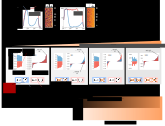
\includegraphics[width=\textwidth]{figures/Figures_signal_decoding_weber_law}
		\phantomsubcaption
		\label{fig:decoding_a}
	\end{subfigure}
	\begin{subfigure}[t]{0\linewidth}
		\phantomsubcaption
		\label{fig:decoding_b}
	\end{subfigure}
	\begin{subfigure}[t]{0\linewidth}
		\phantomsubcaption
		\label{fig:decoding_c}
	\end{subfigure}
	\caption{\footnotesize{Input adaptation aids robust odor signal reconstruction through a wide range of odor concentration changes. \textbf{A} Percent correctly decoded odors, with (red) and without (blue) Weber Law adaptation. For both a homogeneous and diverse receptor repertoire, odor decoding is preserved over background changes in the adaptive system. Heatmaps of $K^*_{ia}$ matrices illustrate receptor homogeneity for the two systems. \textbf{B} Dependence of decoding accuracy on odor sparsity. At low concentrations, both systems can decode relatively complex signals; as concentration increases, complex signals are mis-identified in the absence of adaptive feedback. \textbf{C} Separation of intensity and identity decoding. At low concentrations, both signal identity and intensity are correctly inferred in a non-adaptive system. Increases in signal concentrations can lead to errors in odor intensity, identity, or both. When Weber Law is enforced, the representation of odor intensity and its identity are maintained through a wide regime of odor concentrations.}}
	\label{fig:decoding}
\end{figure*}

To incorporate the linear framework of compressed sensing into our nonlinear encoding model, we treat the odor encoding process exactly, while approximating the decoding to first order. %The latter assumption allows the compressed sensing algorithm -- a constrained optimization problem -- to remain convex, whereby the global minimum is unique. 
Specifically, we represent the nonzero components $s_k$ of the sparse odor signal as $s_k = s_0 + \Delta s_k$, where $s_0$ is the center of the linearization. The target of the decoding process are the identities and intensities of the `excess' signals $\Delta s_i$. 
%The `excess' Or/Orco activity is then defined as:
%\begin{align}
%\Delta \bar A_a \equiv \bar A_a(\mathbf s) - \bar A_a(\mathbf s_0),
%\end{align}
%where we have assumed that the neural system has access to a baseline odor signal $\mathbf s_0$, but must infer exact odor concentrations $s_k$. The decoding process minimizes the the $L_1$ norm of $\Delta s_i$, equivalent to enforcing signal sparsity, while enforcing the linear constraints arising from the excess activities, i.e. the ORN responses. 
To assess the decoding performance, we denote an odor signal as accurately decoded if (i) the sparse odorant components are all estimated to within 25\% of their correct value and (ii) the components absent in the original signal ("zero" components) are all estimated as less than 10\% of the mean excess concentration, $\hat s_j \le \langle \Delta s_k \rangle$. The former is a measure of accurately inferring signal \textit{intensity}; the latter of signal \textit{identity}. 

We apply this scheme to receptor systems consisting of 50 Or/Orco complexes interacting with a 100-dimensional odorant space. Without adaptive feedback, nearly all 100 random sparse odor signals (each odor has $7$ nonzero odorants) are still correctly inferred in a particular regime of mean odor concentration (Fig.~\ref{fig:decoding_a}; blue curves). We find that this holds true for two distinct neural systems, one of which contains homogeneously but all broadly responding receptors (for each $a$, $K^*_{ia}$ are sampled from the same distribution), the second of which is more indicative of \textit{Drosophila} physiology and exhibits a diverse repertoire ranging from broad to highly specialized (as in Fig.~\ref{fig:tuning_curves}). In both cases, however, decoding fidelity is not concentration invariant, dropping sharply outside this regime of faithful signal decoding.

Conversely, we hypothesize that by stabilizing the excess activity levels through Weber-Fechner adaptive feedback, such sensitivity can be mitigated. Enforcing this scaling law above a mean odor concentration of $\langle s_i \rangle~=~10^{-1}$, and matching $\epsilon_a$ to the unadaptive system otherwise, we find that coding fidelity is now maintained over a five-fold change (a.u.) in odor concentration (Fig.~\ref{fig:decoding_a}; red curves). %We further illustrate this behavior for systems with odorant binding distributions that are chosen exponentially and normally ({\color{blue} Supplementary; to be added}). 
This invariance holds across differing levels of signal sparsity (Fig.~\ref{fig:decoding_b}). In the adaptive system, signals with complexity as high as 10 odorants are robustly decoded over several orders of odor concentration. In the non-adaptive system even mono-molecular signals are mis-identified at increased concentrations, a consequence of response homogenization across the ORN repertoire.


A critical feature of olfactory systems is the ability to simultaneously decode odor intensity and identity, aspects which can in principle overlap~\cite{intensity_vs_identity, segregation_intensity_identity}. Compressed decoding conflates these two aspects into a single computation by inferring not only the exact component magnitudes of an odor signal (intensity), but also which molecular components constitute the high-dimensional signal in the first place (identity). Despite the conflation of these in practice, it is possible that in this framework, one aspect may be preserved while the other is violated. 

Separating errors in odor intensity from those in error identity, we find that for an un-adaptive system, either or both may contribute depending on odor concentration. For moderate concentrations, the inferred zero components reach a substantial fraction of the mean odor concentration, while the estimates of the sparse components are largely even with their true values -- the identity of the odor is compromised (Fig.~\ref{fig:decoding_c}). As concentrations increase further, identity is now preserved (zero components are estimated well below the mean), but errors in odor intensity have magnified. This illustrates that in the absence of front-end gain control, errors both in identity and intensity can confound odor representations, while Weber Law feedback can mitigate these conflicts. 



%%%%%%%%%%%%%%%%%%%%%%%%%%%%%%%%%%%%%%%%%%%%%%%%%%%%%%%%%%%%%%%%%
%%%%%%%%%%%%		INHIBITORY NORMALIZATION		%%%%%%%%%%%%%
%%%%%%%%%%%%%%%%%%%%%%%%%%%%%%%%%%%%%%%%%%%%%%%%%%%%%%%%%%%%%%%%%



\subsection{Inhibitory normalization}



{\color{blue} forthcoming; perhaps put this in previous section and relegate figures to SI?}


%%%%%%%%%%%%%%%%%%%%%%%%%%%%%%%%%%%%%%%%%%%%%%%%%%%%%%%%%%%%%%%%%
%%%%%%%%%%%%		NORMALIZATION  FIGURE			%%%%%%%%%%%%%
%%%%%%%%%%%%%%%%%%%%%%%%%%%%%%%%%%%%%%%%%%%%%%%%%%%%%%%%%%%%%%%%%



\begin{figure}
	\begin{subfigure}[t]{\linewidth}
		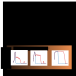
\includegraphics[width=\textwidth]{figures/Figures_signal_decoding_weber_law_2}
		\phantomsubcaption
		\label{fig:divisive_normalization_a}
	\end{subfigure}
	\begin{subfigure}[t]{\linewidth}
		\phantomsubcaption
		\label{fig:divisive_normalization_b}
	\end{subfigure}
	\caption{\textbf{A} Schematic of divisive normalization / lateral inhibition \text{B} Increasing divisive normalization w and w/o Weber Law}
	\label{fig:divisive_normalization}
\end{figure}



%%%%%%%%%%%%%%%%%%%%%%%%%%%%%%%%%%%%%%%%%%%%%%%%%%%%%%%%%%%%%%%%%
%%%%%%%%%%%%		ODOR DISCRIMINATION             %%%%%%%%%%%%%
%%%%%%%%%%%%%%%%%%%%%%%%%%%%%%%%%%%%%%%%%%%%%%%%%%%%%%%%%%%%%%%%%



\subsection{Weber Law scaling aids odor discrimination in conflicting environments}


Olfactory sensing in naturalistic settings relies on the ability to discriminate multiple odors, which may differ or overlap in chemical makeup and intensity. Though Weber Law adaptation can preserve decoding accuracy over changes in odor intensity, a system which adapts to mean concentrations alone may well fail in the presence of distinct odors of differing concentrations. To test this, we consider two sparse odors. The first we call the ``foreground" odor, and hold its component concentrations fixed at $s_{0, \text F} + \Delta s_{k, \text F}$; $s_{0, \text F} = 1$ and $\Delta s_{k, \text F} = 0.2$. The second, which can span intensities a few orders below or above $s_{k, \text F}$, we refer to as the ``background" odor, investigating how its intensity and complexity can affect the identification of the foreground signal. We maintain the total nonzero components of the signal at 7, but split these seven components between the two odors in increasing ratios. 

We first find that molecularly complex backgrounds, if sufficiently strong, can confuse the identification of single odorant foregrounds, both for adaptive and non-adaptive systems (Fig.~\ref{fig:signal_discrimination_a}). Still, the adaptive case is more robust to decoding errors, maintaining accuracy to a higher concentration. Meanwhile, the background odor is now misidentified in the non-adaptive system, until its concentration has sufficiently surpassed the simpler foreground~(Fig.~\ref{fig:signal_discrimination_e}). Importantly, there is no regime in which both odors are correctly identified by a non-adaptive system. Conversely, enforcing Weber's Law robustly identifies both odors in a window of concentrations between 1e-1 to 1e0 (a.u.), suggesting that adaptive feedback can aid odor discrimination in conflicting odor environments.

When the foreground odor consists of more molecular constituents (but is still less complex than the background), it is more robustly decoded in a non-adaptive system (Fig.~\ref{fig:signal_discrimination_d}); however, the foreground signal is more commonly mis-estimated~(Fig.~\ref{fig:signal_discrimination_c}). This pattern continues as the complexity of the odors are about equal (Fig.~\ref{fig:signal_discrimination_e} and Fig.~\ref{fig:signal_discrimination_f}). Meanwhile, the accuracy of the adaptive system remains relatively robust, and its window of accurate odor discrimination has increased. Finally, we find that odors are most easily discerned amid backgrounds of varying concentrations when these backgrounds are molecularly simple (Fig.~\ref{fig:signal_discrimination_g} and \ref{fig:signal_discrimination_h}). While a window of faithful odor discrimination has appeared in the non-adaptive system, this regime is markedly larger in the adaptive case.

Together, these results suggest that in some cases a non-adaptive system of distributed receptors can still discriminate two odors of differing concentrations, but accuracy is sensitive to odor complexity. Conversely, by adapting receptor gain to the mean odor concentration in accordance with Weber's Law, discrimination accuracy is robustly maintained over a large range of odor concentrations and relative molecular complexities. 


%%%%%%%%%%%%%%%%%%%%%%%%%%%%%%%%%%%%%%%%%%%%%%%%%%%%%%%%%%%%%%%%%
%%%%%%%%%%%%      ODOR DISCRIMINATION FIGURE        %%%%%%%%%%%%%
%%%%%%%%%%%%%%%%%%%%%%%%%%%%%%%%%%%%%%%%%%%%%%%%%%%%%%%%%%%%%%%%%



\begin{figure*}[!tb]
	\begin{subfigure}[t]{\linewidth}
		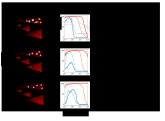
\includegraphics[width=\textwidth]{figures/Figures_signal_discrimination_weber_law}
		\phantomsubcaption
		\label{fig:signal_discrimination_a}
	\end{subfigure}
	\begin{subfigure}[t]{0\linewidth}
		\phantomsubcaption
		\label{fig:signal_discrimination_b}
	\end{subfigure}
	\begin{subfigure}[t]{0\linewidth}
		\phantomsubcaption
 		\label{fig:signal_discrimination_c}
	\end{subfigure}
	\begin{subfigure}[t]{0\linewidth}
		\phantomsubcaption
		\label{fig:signal_discrimination_d}
	\end{subfigure}
	\begin{subfigure}[t]{0\linewidth}
		\phantomsubcaption
		\label{fig:signal_discrimination_e}
	\end{subfigure}
	\begin{subfigure}[t]{0\linewidth}
		\phantomsubcaption
		\label{fig:signal_discrimination_f}
	\end{subfigure}
	\begin{subfigure}[t]{0\linewidth}
		\phantomsubcaption
		\label{fig:signal_discrimination_g}
	\end{subfigure}
	\begin{subfigure}[t]{0\linewidth}
		\phantomsubcaption
		\label{fig:signal_discrimination_h}
	\end{subfigure}
	\caption{\footnotesize{Input adaptation promotes discrimination of distinct odors across conflicts in molecular complexity. \textbf{A/B}~Percentage of correctly decoded sparse odor signals with 7 nonzero components, each consisting of a 1-component foreground odor at a concentration of $s_{k, \text F} \sim 1$ and a 6-component background odor, as a function of background odor intensity. The estimate for the foreground odor components are shown in (A); the background components in (B), averaged over 100 odor identities; non-adaptive system plotted in blue and adapting system in red. \textbf{C-H}~Corresponding plots for foreground/background component ratios of 2:5, 4:3, and 6:1.}}
	\label{fig:signal_discrimination}
\end{figure*}

%When the odor complexities are matched, the regime in which the foreground is correctly decoded has reduced substantially. Further, in the non-adaptive system, in only in a small range of background concentrations can both odors be simultaneously decoded accurately. This behavior magnifies as the foreground becomes more complex (Fig.~\ref{fig:signal_discrimination}). We conclude that adaptive feedback, when incorporated in a combinatorial coding scheme, aids the robust odor discrimination despite disparities in molecular complexity and intensity. 



%%%%%%%%%%%%%%%%%%%%%%%%%%%%%%%%%%%%%%%%%%%%%%%%%%%%%%%%%%%%%%%%%
%%%%%%%%%%%%	   	   TEMPORAL CODING                %%%%%%%%%%%
%%%%%%%%%%%%%%%%%%%%%%%%%%%%%%%%%%%%%%%%%%%%%%%%%%%%%%%%%%%%%%%%%



\subsection{Dynamic adaptation preserves active odor perception in fluctuating odor environments}
So far, we have assumed that odor signals are static in time, and that adaptation from the neural circuitry feeds back onto the receptor sensitivity instantly and perfectly. But realistic odor environments are highly intermittent and widely fluctuating, exhibiting odor concentrations that can span several orders~\cite{celani}. Further, limitations on energy consumption can limit adaptation speed and accuracy~\cite{ESA}. To account for temporal aspects in both the odor environment and sensing periphery, we relax the assumption that adaptation is instantaneous, instead letting the activity of each Or/Orco complex decay linearly to baseline levels $\bar{A}_{a, 0}$ via accompanying modulation of the complex free energies. Specifically, in response to a dynamic odor signal $s(t)$, the activity of complex $a$ is still given by Eq.~\ref{eq:steady_state_act}, but now with time-dependent free energies, $\epsilon_a \rightarrow \epsilon_a(t)$ obeying the dynamics
\begin{align}
\frac{d\epsilon_a(t)}{dt} &= \frac{1}{\tau_a}\left[\bar{A}_a - \bar {A}_{a,0}\right],
\label{eq:WL_dynamics}
\end{align}
where $\bar {A}_a = \bar{A}(s(t), \epsilon_a(t))$ is the time-dependent activity level and $\tau_a$ sets the timescale of adaptation. We compare the results for several timescales between 10 ms and several seconds. In accordance with out assumption that the adaptive mechanism acts on the universal co-receptor Orco, we assume that the adaptation timescale is receptor-independent, $\tau_a \equiv \tau$. 



%%%%%%%%%%%%%%%%%%%%%%%%%%%%%%%%%%%%%%%%%%%%%%%%%%%%%%%%%%%%%%%%%
%%%%%%%%%%%%	   	   TEMPORAL FIGURE                %%%%%%%%%%%
%%%%%%%%%%%%%%%%%%%%%%%%%%%%%%%%%%%%%%%%%%%%%%%%%%%%%%%%%%%%%%%%%



\begin{figure*}[!tb]
	\begin{subfigure}[t]{\linewidth}
		{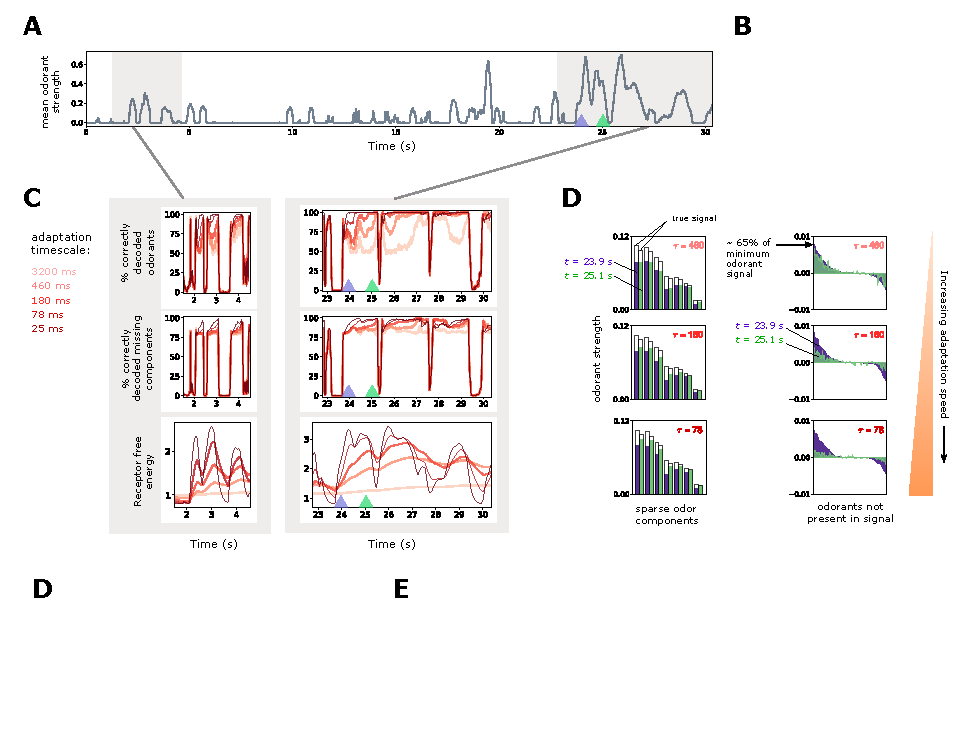
\includegraphics[width=\linewidth]{figures/Figures_temporal_coding}}
		\phantomsubcaption
		\label{fig:temporal_coding_a}
	\end{subfigure}
	\begin{subfigure}[t]{0\linewidth}
		\phantomsubcaption
		\label{fig:temporal_coding_b}
	\end{subfigure}
	\begin{subfigure}[t]{0\linewidth}
		\phantomsubcaption
		\label{fig:temporal_coding_c}
	\end{subfigure}
	\begin{subfigure}[t]{0\linewidth}
		\phantomsubcaption
		\label{fig:temporal_coding_d}
	\end{subfigure}
	\begin{subfigure}[t]{0\linewidth}
		\phantomsubcaption
		\label{fig:temporal_coding_e}
	\end{subfigure}
	\caption{\footnotesize{Dynamic front-end adaptation aids active perception of odor identity in naturalistic odor environments. \textbf{A}~Time course of mean odor signal concentration $s_0$. \textbf{B}~By row, percentage of correctly decoded nonzero components of sparse odors, percentage of correctly decoded zero components, and receptor activation energies $\epsilon_a$, throughout the time course of two distinct regions containing various whiffs, for adaptation timescales range from long (light red) to short (dark red). Percentages are determined by averaging over 20 distinct estimated odor identities. \textbf{C}~Estimates of the sparse components of one of the 20 odor identities at the beginning and end of the whiff denoted by the purple and green markers in (A) and (B), for different adaptation timescales. \textbf{D}~Estimates of zero components of the odor signal corresponding to the same whiff, odor identity, and timescales as in (C). Odor components (which should be zero) are ordered by magnitude of estimate at whiff onset (purple); some components are mis-estimated to be as high as 2/3 of the smallest component of the sparse odor. \textbf{E}~Errors in sparse and zero components of odor signals as a function of adaptation rate, averaged over all 20 odor identities and all whiff encounters, determined by a threshold concentration of 0.1 (a.u.)}}
	\label{fig:temporal_coding}
\end{figure*}

Next, to mimic a naturalistic odor signal, we used recorded traces from a photo-ionization detector whose statistics were verified to match those of natural odor plumes (Fig.~\ref{fig:temporal_coding_a}). The signals was scaled to concentrations applicable to our model framework.

Considering first a set of 100 randomly chosen sparse odors of unique identities, we plot in Fig.~\ref{fig:temporal_coding_b} decoding errors arising from either mis-identification of odor identity, or that of odor intensity, in two windows containing odor whiffs. %Specifically, we plot, over time, the percentage of correctly estimated nonzero component intensities, as well as the the percentage of correctly identified zero components $s_k$, for several distinct adaptation timescales. 
For slow adaptation, with timescales greater than a few hundred ms (lighter curves in Fig.~\ref{fig:temporal_coding_b}), we find clear trends in both intensity and identity coding. Errors in odor intensity are quite sensitive to the faster fluctuations in the odor signal, even if the signal remains appreciable throughout the whiff. While 80\% of the odorant identity is perceived immediately at whiff threshold, the estimate accuracy fails to improve from then onward through the duration of the whiff. Conversely, with faster adaptation ($\tau < 100$ ms), the coding of odor intensity corrects within the first 100 ms of the whiff onset (dark red curves). Interestingly, odor intensity coding improves steadily as the whiff endures, though it takes several times the adaptation timescale to minimize the errors. 



%%%%%%%%%%%%%%%%%%%%%%%%%%%%%%%%%%%%%%%%%%%%%%%%%%%%%%%%%%%%%%%%%
%%%%%%%%%%%%	   	   TEMPORAL FIGURE 2              %%%%%%%%%%%
%%%%%%%%%%%%%%%%%%%%%%%%%%%%%%%%%%%%%%%%%%%%%%%%%%%%%%%%%%%%%%%%%



\begin{figure}[!tb]
	\begin{subfigure}[t]{\linewidth}
		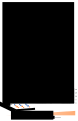
\includegraphics[width=\textwidth]{figures/Figures_temporal_coding_2}
		\caption{blah}
		\label{fig:temporal_coding_2_a}	
	\end{subfigure}
	\begin{subfigure}[t]{0\linewidth}
		\phantomsubcaption
		\label{fig:temporal_coding_2_b}
	\end{subfigure}
	\begin{subfigure}[t]{0\linewidth}
		\phantomsubcaption
		\label{fig:temporal_coding_2_c}
	\end{subfigure}
	\caption{Dynamic adaptation maintains signal decoding fidelity amid fluctuating backgrounds at disparate timescales.}
	\label{fig:temporal_coding_2}
\end{figure}


%While the number of mis-identified zero components during whiffs may appear minor (20\% or so), this corresponds to several times the number of sparse components defining the odor signal itself, which is 7. Thus we expect that the increase from 80\% to $>$95\% through the duration of the whiff indeed corresponds to a salient, dynamically improving perception of odor identity. 

To illustrate this in more detail, we consider the errors for only one of the 20 sparse signals, at the onset and closure of the whiff demarcated by the purple and blue markers in Fig.~\ref{fig:temporal_coding_a} and \ref{fig:temporal_coding_b}. In Fig.~\ref{fig:temporal_coding_c}, we plot estimates of the nonzero components of the sparse odor signal at whiff onset and whiff closure for the timescales $\tau = 460$, 180, and 78. For higher adaptation rates, there is some improvement in the estimate of odor intensity by the end of the whiff, but the gains are rather small. On the other hand, the perception of odor identity is particularly frustrated by slow adaptation. For $\tau = 460$, the fraction of zero odor components perceived at $>$10\% of the mean odor signal $\langle \Delta s_k \rangle$ is substantial at whiff onset, and remains unchanged by the end of the whiff (Fig.~\ref{fig:temporal_coding_d}). For $\tau = 78$, the mis-estimated proportion is equivalent at whiff onset, but has vanished by whiff end. This is further corroborated by averaging over all whiffs (Fig.~\ref{fig:temporal_coding_e}). Together, this illustrates that dynamic front-end adaptation to mean signal intensity actively aids the perception of odor identity in intermittent odor environments. 


Finally we ask: Can adaptive feedback can actively improve the the perception of odor identity in the presence of dynamic adaptation, fluctuating odors \textit{and} fluctuating backgrounds? We consider three cases, in which a background odor modulates on timescales roughly that of the foreground, somewhat slower, and substantially slower. To maximize potential conflicts, we assume the foreground and background odors span odor intensities of roughly equal magnitude. In addition, anticipating our earlier results (Fig.~\ref{fig:signal_discrimination}), we consider various levels of relative complexity among these two odors. %{\color{blue} Explain how performanec is quantified}

When the timescale of background fluctuations is long, we find that performance improves markedly with adaptation speed (mis-identified zero components drop from 14 to 0 as timescale varies from 10 seconds to 0.5 seconds), but is already maximized at 500 ms, which exceeds the duration of most of the odor whiffs. In other words, contrary to the single odor case, odors are perfectly identified even when adaptive gain operates at timescales somewhat slower than the signal fluctuations. For slightly faster background fluctuations, but still slower than the foreground timescale, we see a marked degradation in performance with slower adaptation, although again the performance largely saturates at timescales of 500 ms or so. Further, there is now a strong dependence on foreground complexity; simpler foregrounds are easier to perceive above the background (number of mis-identified zero components $\sim 3$), while very complex foregrounds have a larger number of misidentified components $\sim 8$. This pattern continues when the background fluctuates as quickly as the foreground, though the performance  is only slightly degraded. Importantly, there is a monotonic gain in performance as adaptation speed increases, holding across fluctuation timescales and molecular complexity. Our key finding is that for odors that fluctuate on well-separated timescales, dynamic adaptive feedback obeying the Weber-Fechner Law and operating moderately quickly promotes the active perception of odor identity. 


\section{Discussion}

Drawing on recent evidence for the existence of the Weber-Fechner law in in \textit{Drosophila} olfactory receptor neurons~\cite{cafaro_WL, cao_WL,  srinivas_elife}, we propose a theoretical framework for the adaptive encoding and decoding of complex, dynamic odor environments. We argue that this adaptive mechanism, when incorporated into a combinatorial coding strategy, is central to the accurate identification and discrimination of rapidly fluctuating, potentially conflicting odor signals. Our framework relies on two steps of odor encoding and decoding, respectively: (i) a nonlinear, stochastic model of odor-receptor binding and subsequent receptor activity, and ii) reconstruction of the signal via compressed decoding of the neural response. In this framework, input gain control following the Weber-Fechner Law is enforced by appropriate scaling of the free energy of Or/Orco complex activation with the odor signal mean. 

The encoding model is a generalization of the classical model of bacterial chemotaxis~\cite{tu_shimizu_berg}, and is mathematically equivalent to a recently proposed competitive binding model for ORN response~\cite{Cao_Tu_WL}, where it was shown that inclusion of inhibitory responses increases coding capacity of a distributed system of ORNs. Regarding decoding, recent works have pointed to the importance of a distributed response in inferring high-dimensional sparse signals~\cite{vijay_1, vijay_2, sharpee_zhang}. In this work, we place particular importance on the impact of intensity variations that typify odor signals in natural environments, finding that in both static and fluctuating odor landscapes, adaptive sensing at the receptor level play a central role in the simultaneous decoding of odor intensity and odor identity. 


\subsection{Maintaining a distributed response}

We showed that for static odor signals, a broadly sensing but non-adaptive system can accurately estimate odor identities, though only in a limited window of concentration. In living systems, adaptation maintains information transfer by ensuring that the sensory system stays in a regime of maximum sensitivity~\cite{information_theory_adaptation}. In compressed sensing, the fidelity of signal decoding relies also on the combinatorics of the sensor response~\cite{CS_tao, CS_donoho, CS_ganguli}. Indeed, it has been noted that \textit{diffusivity} in sensing -- here incorporated through the dispersity of binding constants -- underlies effective compression of high-dimensional sparse signals into a limited receptor space. Still, the nonlinearity of the steady state receptor response, Eq.~\ref{eq:steady_state_act}, can affect the distributions of ORN activity as odor concentration increases. Thus, in the context of combinatorial coding, the central benefit conferred by the Weber Law scaling is not merely preventing ORN activities from saturating, but their distributions from distorting. 

Importantly, we find that the advantages of preserving combinatorial response carry over to more complex odor environments, where multiple odors must be discriminated. The ability to recognize weak odors over strong backgrounds is particularly relevant to olfaction in nature, where signal conflicts are pervasive. Absent Weber Law scaling, odor signals are mis-identified in the presence of strong backgrounds, producing accurate estimations only beyond a minimum intensity; this minimum itself increases with odor complexity. Further, the system is largely incapable of estimating both odors accurately -- true discrimination -- except in limited concentration windows. In principle, the adaptive system might also be susceptible to signal conflicts: mathematically, the activity distributions are invariant only in the limit that all odorants are of equal strength (Eq), so the large deviations of the weaker odorant concentrations from this mean value could lead to sensitive distortions in the distribution of ORN activities. Nonetheless, we find that odors at least as strong as the background can be identified irrespective of odor complexities. Likewise discrimination accuracy is more robust, preserved over sizable concentration windows. 


%\subsection{Relative abundances of ORN classes}
%We tested our model on a particular combination of odor sparsity, odorant dimension, and receptor dimension, for various choices of system $K^*_{ia}$ and odor identity. One aspect as yet unexplored is the relative distribution of different receptor types. Though ORNs of a given type project to a single glomerulus in the antennal lobe, multiplicities of one ORN class over another may still affect information transfer. The optimality of a non-uniform receptor distribution in some environments was recently demonstrated for a linear combinatorial sensing system; a suggestive extension of this work is investigating {\color{blue} Say some more about future experiments or something}


\subsection{Simultaneous coding of intensity and identity}

An important aspect of olfactory sensing is maintaining fidelity in encoding odor identity simultaneously with that of odor intensity~\cite{intensity_vs_identity}. Here we find that in some situations these aspects may decouple with variations in odor environment; often, though errors in one coincide with errors in the other. As mentioned, compressed sensing naturally conflates identity and intensity, decoding the exact strength of odor signal components while relying fundamentally on the requirement that most of components are zero. In this sense, combinatorial coding and compressed sensing decoding confronts the identity-intensity dilemma quite naturally, perhaps moreso than in sensory systems in which stimuli are parameterized continuously (e.g. by frequency), such as vision and audition. Still, evidence suggests that, at least in \textit{Drosophila}, odor and intensity may be encoded in distinct regions in the mushroom body~\cite{segregation_intensity_identity}, so incorporating a more realistic neural model for decoding of sparse ORN response (such as in~\cite{sharpee_zhang}) may find that these two aspects naturally segregate.

%An intriguing result in our framework is the distinct manner in which errors in intensity and identity diminish during the active perception of an odor whiff. Even for relatively long adaptive timescales, identity perception increases monotonically as the odor persists, insensitive to ongoing fluctuations. Further, the proportion of mis-identified odorants continues falling on timescales much longer than $\tau$. 

\subsection{Divisive normalization / timescales}
{\color{blue} TODO}

\subsection{The timescales of adaptation mechanisms}

We find that in naturalistic, intermittent odor environments, dynamic adaptation can promote active perception of sparse odors throughout whiffs. In particular, adaptation timescales around 100 ms are sufficient in maintaining ongoing refinements of perceived odor identity, and that these refinements confer robust and accurate odor identification within a short time ($<$500 ms) following whiff onset. We also find that sufficiently rapid adaptation aids odor intensity coding, although these gains are not as stark. Finally, dynamic adaptation can promote the accurate detection of fluctuating odors within background environments whose intensity variations are sufficiently slow. 



Several studies have implicated the importance of ORN temporal dynamics in odor encoding~\cite{multiple_timescales_stopfer, primacy_coding, olfactory_coding_latency, chih-ying, martelli, odor_coding_rate_verhagen, neural_network_temporal_coding, dweck}. In mammalian olfaction, recent studies raise the possibility that the few most sensitive ORs are solely responsible for coding odor identity, a so-called "primacy code"~\cite{primacy_coding}; such a representation is concentration invariant, as higher intensities would recruit the response of other, less sensitive receptors, but still retain this particular subset. While our results implicate \textit{all} ORNs, not just the most sensitive, in faithful odor encoding~\cite{vijay_1}, there are several reasons to believe these two viewpoints are not inconsistent (aside from anatomical differences between the mammalian and insect olfactory periphery~\cite{mammalian_olfaction}). First, combinatorial coding applies to the identification of complex mixtures, not single odorants as tested in~\cite{primacy_coding}. Second, while many odors may be encoded by distributed activity patterns in ORNs and corresponding glomeruli, some odors relevant for innate behaviors such as mating and feeding may contain their own dedicated pathways; these latter odors may rely on strong, specialized responses~\cite{dweck, evolution_insect_olfaction}. The presence of broad and narrowly tuned olfactory receptors in \textit{Drosophila} suggests that both combinatorial and primacy coding play distinct, complementary roles in naturalistic odor sensing. 







\section{Online Methods}

\subsection{Stochastic odor-receptor binding model}

We model an odor as an $N$-dimensional vector $\mathbf s = \langle s_1,...,s_N\rangle$, where $s_i > 0$ are the concentrations of individual volatile molecules (odorants) comprising the odor. In addition, we assume that the odors are sparse in the space of odorants, so only $K$ components of $\mathbf s$ are nonzero, where $K \ll N$. The olfactory sensory system is modeled as a collection of $M$ distinct Or/Orco complexes, each of which can be bound with any one of the odorant molecules, and can be either active (firing) inactive (quiescent). We only consider competitive binding, so a complex is bound with one odorant at most. With $N$ possible odorants, receptor $a$ resides in one of $2N+2$ possible states, \{$R_a$, $R^*_a$, $R_a$-$s_i$, $R^*_a$-$s_i$\}, indicating receptors that are unbound/inactive, unbound/active, inactive/bound to odorant $i$, and active/bound to odorant $i$, respectively. Unless otherwise indicated, we set $N = 100$, $K = 7$, and $M = 50$ throughout.

The system dynamics are schematized in Fig.(). In the mean-field limit, the binding dynamics of these $2N + 2$ states are described by the master equations:

\begin{align}
\frac{d[R_a\text{-}s_i]}{dt} &= k^+_{ia}s_i[R_a] - k^-_{ia}[R_a\text{-}s_i] \label{eq:Meq_inactive_bind_rate}\\
\frac{d[R^*_a\text{-}s_i]}{dt} &= k^{*+}_{ia}s_i[R^*_a] - k^{*-}_{ia}[R^*_a\text{-}s_i],
\label{eq:Meq_active_bind_rate}
\end{align}
when receptor $R_a$ is either inactive (Eq.~\ref{eq:Meq_inactive_bind_rate}) or active (Eq.~\ref{eq:Meq_active_bind_rate}). Further, transitions between inactive and active states are described in the mean limit via:
\begin{align}
\frac{d[R_a]}{dt} &= w^{\text{u}+}_a [R_a] - w^{\text{u}-}_a [R^*_a] \label{eq:Meq_unbound_active_rate}\\
\frac{d[R^*_a\text{-}s_i]}{dt} &=  w^{\text{b}+}_{ia} [R_a\text{-}s_i] - w^{\text{b}-}_{ia}  [R^*_a\text{-}s_i],
\label{eq:Meq_bound_active_rate}
\end{align}
when receptor $R_a$ is either unbound (Eq.~\ref{eq:Meq_unbound_active_rate}) or bound (Eq.~\ref{eq:Meq_bound_active_rate}). The corresponding disassociation constants in terms of the binding transition rates are:


\begin{align}
K_{ia} = \frac{k^-_{ia}}{k^+_{ia}} \nonumber \\
K^*_{ia} = \frac{k^{*-}_{ia}}{k^{+*}_{ia}} 
\label{eq:Kd}
\end{align}

Following~\cite{srinivas_elife}, we assume that in steady state, the active firing state of an Or/Orco complex is energetically suppressed from the inactive state through corresponding Boltzmann factors:

\begin{align}
\frac{[R^*_a]}{[R_a]} &= \frac{w^{\text{u}+}_a}{w^{\text{u}-}_a} \equiv e^{-\epsilon_a} \label{eq:epsilon_unbound} \\
\frac{[R^*_a\text{-}s_i]}{[R_a\text{-}s_i]} &= \frac{w^{\text{b}+}_{ia}}{w^{\text{b}-}_{ia}} \equiv e^{-\epsilon^{\text b}_{ia}}.\label{eq:epsilon_bound}
\end{align}
These energies are related through detailed balance, which we assume. Applying detailed balance to a given 4-cycle as in Fig.~() gives
\begin{align}
\frac{w^{\text{u}+}_a}{w^{\text{u}-}_a}\frac{k^{*+}_{ia}}{k^{*-}_{ia}}\frac{w^{\text{b}-}_{ia}}{w^{\text{b}+}_{ia}}\frac{k^{-}_{ia}}{k^{+}_{ia}} \equiv 1,
\label{eq:detailed_balance}
\end{align}
which, in conjunction with Eqs.~\ref{eq:Kd}, \ref{eq:epsilon_unbound}, and \ref{eq:epsilon_bound}, gives
\begin{align}
\epsilon_{ia}^{\text b} = \epsilon_a + \ln\left[\frac{K^*_{ia}}{K_{ia}}\right].
\label{testing_equation}
\end{align}
Assuming the binding dynamics are fast, then the probability that receptor $a$ is bound by ligand $i$ when inactive and active can be derived from  Eqs.~\ref{eq:Meq_inactive_bind_rate} and \ref{eq:Meq_active_bind_rate} as
\begin{align}
p^{\text b}_{ia} = \frac{s_i/K_{ia}}{1 + \sum_j^Ns_j/K_{ja}} \label{eq:bound_prob_ai_inactive} \\
p^{\text b, *}_{ia} = \frac{s_i/K^*_{ia}}{1 + \sum_j^Ns_j/K^*_{ja}} \label{eq:bound_prob_ai_active}.
\end{align}
The average  activity $A_a$ of complex $a$ is the likelihood that the complex is active, unbound or unbound (equivalantly, the proportion of Or/Orco complexes in a given ORN that are active):
\begin{align}
A_a = \frac{[R^*_a] + \sum_i^N[R^*_a\text{-}s_i]}{[R^*_a] + \sum_i^N[R^*_a\text{-}s_i] + {[R_a] + \sum_i^N[R_a\text{-}s_i]}}.
\end{align} 
Using the master equations between active and inactive states Eq.~\ref{eq:Meq_unbound_active_rate} and \ref{eq:Meq_bound_active_rate}, this activity obeys the master equation
\begin{align}
\frac{dA_a}{dt} &= w^+_a(1 - A_a) + w^-_aA_a
\label{eq:dadt}
\end{align}
with effective transition rates
\begin{align}
w^+_a &= \sum_i^Np^{\text b}_{ia} w^{\text u +}_{ia} + p_{a}w^{\text u}_a 
\end{align}
and analogously for $w_a^-$. Setting Eq.~\ref{eq:dadt} to zero gives the steady state average activity level of ORN $a$:
\begin{align}
\bar{A}_a = \left(1 + e^{\epsilon_a}\frac{1 + \sum_i^N s_i/K_{ia}}{1 + \sum_i^N s_i/K^*_{ia}}\right)^{-1}. \tag{\ref{eq:steady_state_act}}
\end{align}
	
\subsection{Generation of binding matrices $K^*_{ia}$}
$K_{ia}^*$ matrices are generated by sampling at two stages. First, for each receptor complex $a$, the disassociation constants for ligand $i$ were chosen uniformly: $K^*_{ia} \sim \mathcal U[\mu_a, \nu_a]$. Each of these bounds were themselves drawn from a hyperdistribution, also uniform, $\mu_a \sim \mathcal U[\mu_{a, \text L}, \mu_{a, \text H}]$ and $\nu_a \sim \mathcal U[\nu_{a, \text L}, \nu_{a, \text H}]$. $K_{ia}$ matrix elements were set identically to 1e3 throughout. 

\subsection{Odor signals}
Odor signals are $N$-dimensional vectors, $N=100$, presumed sparse whereby only $K$ components, $K \ll N$, are nonzero. 

\subsection{Compressed sensing decoding of ORN response}
We decode ORN responses to infer odor signal identities using an abstraction intended to mimic the neural computations underlying odor identification in the \textit{Drosophila} mushroom body. While we make no assumptions that the compressed sensing (CS) algorithm (or one like it) is being utilized in actuality, this framework nonetheless informs our understanding of how the neural representation of odor identity is maintained or lost when passed through a distributed ORN repertoire. In this sense, CS is somewhat of an upper bound on how well a real neural computation might perform in decompressing ORN responses.

We assume that ORN firing rates are linear in the Or/Orco complex activity; for simplicity we let this transform be the identity. Though subsequent neural circuitry, particularly from the glomeruli in the AL to the Kenyon cells in the MB further mix and scramble these responses, we focus here on the information transfer at the sensory periphery alone. In any case, as demonstrated previously~\cite{vijay_1}, we expect that these neural computations would only improve the representation of neural identity, so we expect no negative ramifications for our findings.

CS addresses the problem of determining a sparse signal from a set of linear measurements, when the number of measurements is less than the signal dimension. Specifically, it is a solution to 
\begin{align}
\mathbf y = \mathbf R\mathbf s
\label{eq:CS_constraints}
\end{align}, where $\mathbf s \in \mathbb{R}^N$ and $\mathbf a\in \mathbb{R}^M$ are vectors of signals and responses, respectively, and $\mathbf R$ is the measurement matrix. Since measurements are fewer than signal components, then $M < N$, whereby $\mathbf R$ is wide rectangular and so Eq.~\ref{eq:CS_constraints} cannot be simply inverted to produce $\mathbf s$. The idea of CS is to utilize the knowledge that $\mathbf s$ is sparse, i.e.g only $K$ of its components, $K \ll N$ are nonzero. Both the measurements and sparsity are thus combined into a single constrained optimization routine:
\begin{align}
\hat s_i = \textup{argmin} \sum_i^N |s_i| \quad \textup{such that } \mathbf y = \mathbf R\mathbf s
\label{eq:CS}
\end{align}
where $\hat s_i$ are the optimal estimates of the signal components and the sum, which is known as the $L_1$ norm of $\mathbf s$ is a natural metric of sparsity. 

Importantly, the $L_1$ norm is a convex operation and the constraints are linear, so the optimization has a unique global minimum. To incorporate the nonlinear response of our encoding model into this linear framework, we assume that the responses are generated through the full nonlinear steady state response, Eq.~\ref{eq:steady_state_act}, but that the measurement matrix needed for decoding uses a linear approximation of this transformation.  Expanding Eq.~\ref{eq:steady_state_act} around $s_0 = s_i - \Delta s_i$ gives
\begin{align}
\bar A_a &\approx \bar A_{a, 0} + \Delta \bar{A}_a \label{eq:CS_act_approx} \\
\Delta \bar{A}_a &= \sum_i^NR_{ia}\big|_{s_0}\Delta s_i \label{eq:CS_dAct_approx}\\
\bar A_{a, 0} &= \frac{\sum_1^N s_0/K_{ia}^*}{\sum_1^N s_0/K_{ia}^* + e^{\epsilon_a}} \label{eq:CS_act0_approx} \\
R_{ia}\big|_{s_0} &=  \frac{e^{\epsilon_a}/K_{ia}^*}{(\sum_i^Ns_0/K_{ia}^* + e^{\epsilon_a})^2},
\label{eq:CS_gain_approx}
\end{align}
where we work in the approximation $K^*_{ia} \ll s_0 << K_{ia}$. We assume that the neural system has access to the linearized response, Eq.~\ref{eq:CS_gain_approx}, but must infer the excess signals $\Delta s_i$ from the excess activity $\Delta \bar A_a$. Corresponding to the CS framework, therefore, $\Delta \mathbf {\bar A} \rightarrow \mathbf y$, $\Delta \mathbf s \rightarrow \mathbf s$, and $R_{ia}\big|_{s_0} \rightarrow \mathbf R$. 

We optimize the cost function using sequential least squares programming, implemented in Python through using the scientific package scipy.

\subsection{Or/Orco  energies of activation $\epsilon_a$ and enforcement of Weber's Law}
Free energies are considered receptor-independent throughout, with the exception of dynamically adaptive system in a temporal odor environment (Figs.~\ref{fig:temporal_coding} and \ref{fig:temporal_coding_2}). To enforce Weber's Law, we assume the receptor activities feed back onto $\epsilon_a$ through the dynamics
\begin{align}
\frac{d\epsilon_a(t)}{dt} &= \frac{1}{\tau_a}\left[\bar{A}_a - \bar {A}_{a,0}\right] \tag{\ref{eq:WL_dynamics}}.
\end{align}
For the static case, adaptation is perfect, whereby Or/Orco activities are pegged to their perfectly adapted values $\bar {A}_{a,0}$. Incorporating this into Eq.~\ref{eq:steady_state_act}, and assuming  $K^*_{ia} \ll s_0 << K_{ia}$, gives
\begin{align}
\bar \epsilon_a &= \ln\left(\frac{1-\bar {A}_{a,0}}{\bar {A}_{a,0}}\right) + \ln\left(\sum_i^N\frac{s_i}{K_{ia}^*}\right).
\label{eq:adapted_epsilon}
\end{align}
Assuming that the excess signals are small, $\Delta s_i \ll s_0$, this gives 
\begin{align}
\epsilon_a \approx \ln(s_0) + \epsilon_{a, 0},
\label{eq:WL_approx}
\end{align} 
where $\epsilon_{a, 0}$ are receptor-dependent constants. In the static case, we choose these constants such $\epsilon_{a}$ in both adaptive and non-adaptive systems are equivalent at a given low concentration, $s_{0, \text L}$.  Below this concentration, we assume adaptation is not in effect, so $\epsilon_a = \epsilon_{a, 0} \equiv \epsilon_{\text {L}}$. 

It is important to note that while the linearized gain Eq.~\ref{eq:CS_gain_approx} utilized by the decoding algorithm appears to rely on $\epsilon_a$, by the above argument $\epsilon_a$ can in principle be determined by firing rates alone. That is, $\epsilon_a$ is inferred in time through integration of Eq.~\ref{eq:WL_dynamics}, which relies only on the current ORN activity and the adapted activity $\bar{A}_{a, 0}$. 

\begin{align}
content...
\end{align}




